\documentclass{VUMIFInfKursinis}
\usepackage{algorithmicx}
\usepackage{algorithm}
\usepackage{algpseudocode}
\usepackage{amsfonts}
\usepackage{amsmath}
\usepackage{bm}
\usepackage{color}
\usepackage{url}



\usepackage{graphicx}

\geometry{right=1.20in}


\lhead{}
\chead{}
\rhead{}
\lfoot{}
\cfoot{\thepage}
\rfoot{} 



% Titulinio aprašas
\university{Vilniaus universitetas}
\faculty{Matematikos ir informatikos fakultetas}
\department{Matematinės Informatikos katedra}
\papertype{Bakalauro baigiamasis darbas}
\title{Rankoje laikomų objektų atpažinimas naudojant TensorFlow.js}
\status{4 kurso 3 grupės studentas}
\author{Marek Rusakevič}
\supervisor{Irus Grinis}
\date{Vilnius \\ \the\year}





\begin{document}
\maketitle

\tableofcontents




\subsection*{Įvadas}
\vspace{10mm}

Gilusis mokymasis per paskutinius metus labai išpopuliarėjo. Populiariausios ir dažniausiai naudojamos bibliotekos darbui su neuroniniais tinklais yra \textit{TensorFlow} ir \textit{Keras}. Šitie įrankiai įsitvirtino giliojo mokymo aplinkoje, nes yra galingi ir patikimi. Bet jie turi didelį trūkumą -- jų nustatymas reikalauja nemažai laiko ir žinių, todėl naujokams šioje srityje nelabai patogu pradėti jais naudotis. Su šia problema padeda susidoroti neseniai pasirodęs \textit{TensorFlow.js}.

\subsection*{Tikslas}

Šio darbo tikslas yra sukonstruoti tinklą naudojant \textit{Keras}, o po to naują biblioteką \textit{TensorFlow.js} ir palyginti konstravimo procesus. Su \textit{Keras} sukonstruosime paprasta tinklą, kuris atpažins mažas \textit{„Lego“} detales. Apžvelgsime būdus normalizuoti paveikslėlius (duomenis), kad būtų pasiektas didesnis atpažinimo procentas. Taip pat tinklą konstruosime bandydami skirtingas architektūras ir palyginsime jų efektyvumą.
\par
Su \textit{TensorFlow.js} konstruosime tinklą, kuris leidžia atpažinti skirtingus objektus. Taip pat bandysime išspręsti papildomą problemą: tinklas gerai atpažįsta objektus, kurie neturi jokios papildomos informacijos paveikslėlio fone, bet jeigu kartu su atpažįstamu objektu yra dar vienas, atpažinimo tikimybė tampa kur kas mažesnė. Bandysime sukonstruot tinklą, kuris ignoruos visą foną ir bandys atpažinti objektą, kuris yra laikomas rankoje. Taip pat išbandysime naują neuroninių tinklų konstravimo būdą -- mokymosi perkėlimą (\textit{Transfer learning}). Su mokymosi perkėlimu neuroninio tinklo apmokymo laikas turėtų sumažėti keliskart.

\subsection*{Uždaviniai}

\begin{itemize}
  \item Sukonstruoti tinklą su \textit{Keras} pagalba, kuris atpažįsta mažas \textit{„Lego“} detales.
  \item Peržiūrėti visų sluoksnių tipus: sąsūkos sluoksnį, didžiausio atmetimo, tirštąjį sluoksnį, atmetimo sluoksnį.
  \item Palyginti skirtingas neuroninio tinklo architektūras.
  \item Sukonstruoti tinklą su \textit{TensorFlow.js} naudojant mokymosi perkėlimą (\textit{Transfer learning}), kurį galima bus apmokyti atpažinti skirtingus objektus, kurie bus laikomi rankoje.
  \item Panaudoti \textit{HandTrack.js} biblioteką rankos atpažinimui vaizde.
\end{itemize} 



\section{Gilusis mokymasis}
\vspace{10mm}


Jeigu norime suprasti kas yra gilusis mokymasis, iš pradžių turime suprasti kas yra dirbtinis intelektas, sistemos mokymasis ir kaip jie susiję tarpusavyje.

\begin{figure}[h!]
\centering
  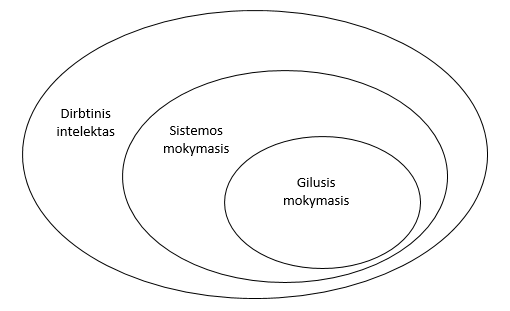
\includegraphics[scale=1.0]{img/figure_1-1}
  \caption{Dirbtinis intelektas, sistemos mokymasis, gilusis mokymasis.}
  \label{fig:AI}
\end{figure}

\subsection{Dirbtinis intelektas (\textit{AI})}

Dirbtinis intelektas buvo pradėtas tyrinėti po Antrojo pasaulinio karo, kai keletas pradedančiųjų kompiuterių srities pionierių pradėjo klausti, ar kompiuteriai galės mąstyti – ir į šį klausimą iki šiol niekas neatsakė.
\par
Trumpas šios srities apibrėžimas būtų toks: pastangos automatizuoti intelektines užduotis, kurias paprastai atlieka žmonės.
\par
AI yra bendra sritis, apimanti sistemos mokymąsi ir gilųjį mokymąsi, tačiau taip pat apima daug daugiau metodų, kurie nereikalauja jokio mokymosi. Pavyzdžiui, ankstyvose šachmatų programose dalyvavo tik programuotojų sukurtos taisyklės. Gana ilgą laiką daugelis ekspertų manė, kad dirbtinio intelekto žmogaus lygmeniu būtų galima pasiekti, sukuriant programuotojų pakankamai aiškių manipuliavimo žinių taisyklių. Šis metodas, žinomas kaip simbolinis AI, buvo dominuojantis nuo 1950 m. iki devintojo dešimtmečio pabaigos. 
\par
Nors simbolinis AI pasirodė esąs tinkamas išspręsti aiškiai apibrėžtas logiškas problemas, tokias kaip žaisti šachmatais Paaiškėjo, kad sunku išsiaiškinti aiškias taisykles, skirtas išspręsti sudėtingesnes, neaiškias problemas, tokias kaip vaizdo klasifikavimas, kalbos atpažinimas ir kalbos vertimas. Sukurtas naujas požiūris į simbolinę AI vietą: sistemos mokymasis. \cite{1}

\subsection{Sistemos mokymasis}

Sistemos, pagrįstos simboliniu dirbtiniu intelektu, negalėjo mokytis iš naujų duomenų. Tai paskatino atsirasti tyrimų sričiai, vadinamai sistemos mokymu, kuri apibrėžiama kaip „kompiuterio apmokymas" iš duotų duomenų, užuot jį tiksliai užprogramavus.
\par
Nors sistemos mokymasis atsirado tik dešimtajame dešimtmetyje, jis greitai tapo daugiausiai naudojama dirbtinio intelekto atmaina. Tą nulėmė padidėjusios duomenų bazės ir galingesni kompiuteriai.


\vspace{10mm}
\begin{figure}[h!]
\centering
  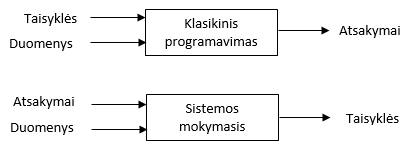
\includegraphics[scale=1.1]{img/figure_1-2}
  \caption{Klasikinis programavimas prieš sistemos mokymąsi.}
\end{figure}
\vspace{10mm}



Klasikiniame programavime programai yra paduodami duomenys ir taisyklės, pagal kurias šie duomenys yra nagrinėjami ir gaunami norimi atsakymai. Su sistemos mokymosi žmonės įveda duomenis, taip pat atsakymus, kurių tikimasi iš duomenų, o gaunamos yra taisyklės. Tada šios taisyklės gali būti taikomos naujiems duomenims pateikti originalius atsakymus. \cite{1}

\subsection{Gilusis mokymasis}

Gilusis mokymasis yra sistemos mokymosi atšaka, kuri naudoja neuroninius tinklus. Neuroninis tinklas yra sudarytas iš kelių sudėtų vienas ant kito sluoksnių, kur kiekvienas sluoksnis išmoksta vis abstraktesnius duomenų bruožus. Gilusis mokymasis vadinamas giliu (\textit{depth of the model}), nes turi daugiau nei kelis sujungtus sluoksnius. Modernus gilusis mokymas dažniausiai turi tarp dešimties ir kelių šimtų sluoksnių, kurie išmoksta bruožus tiesiai iš duomenų.

\vspace{10mm}
\begin{figure}[h!]
\centering
  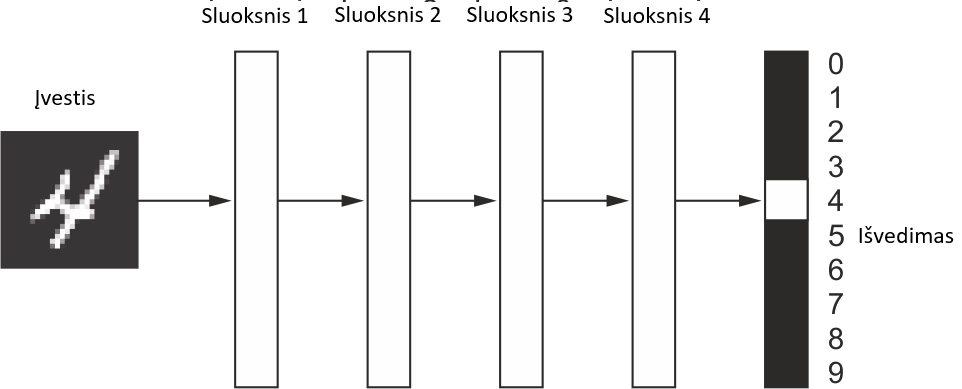
\includegraphics[scale=1.3]{img/figure_1-5}
  \caption{Gilus neuroninis tinklas skaitmenų klasifikacijai.}
  \label{fig:DeepLearningDigit}
\end{figure}

Kaip matome paveikslėlyje \ref{fig:DeepLearningDigit}, tinklas transformuoja pradinį pavekslėlį į reprezentacijas, kurios skiriasi nuo pradinio paveikslėlio ir yra kur kas informatyvesnės.

\begin{figure}[h!]
\centering
  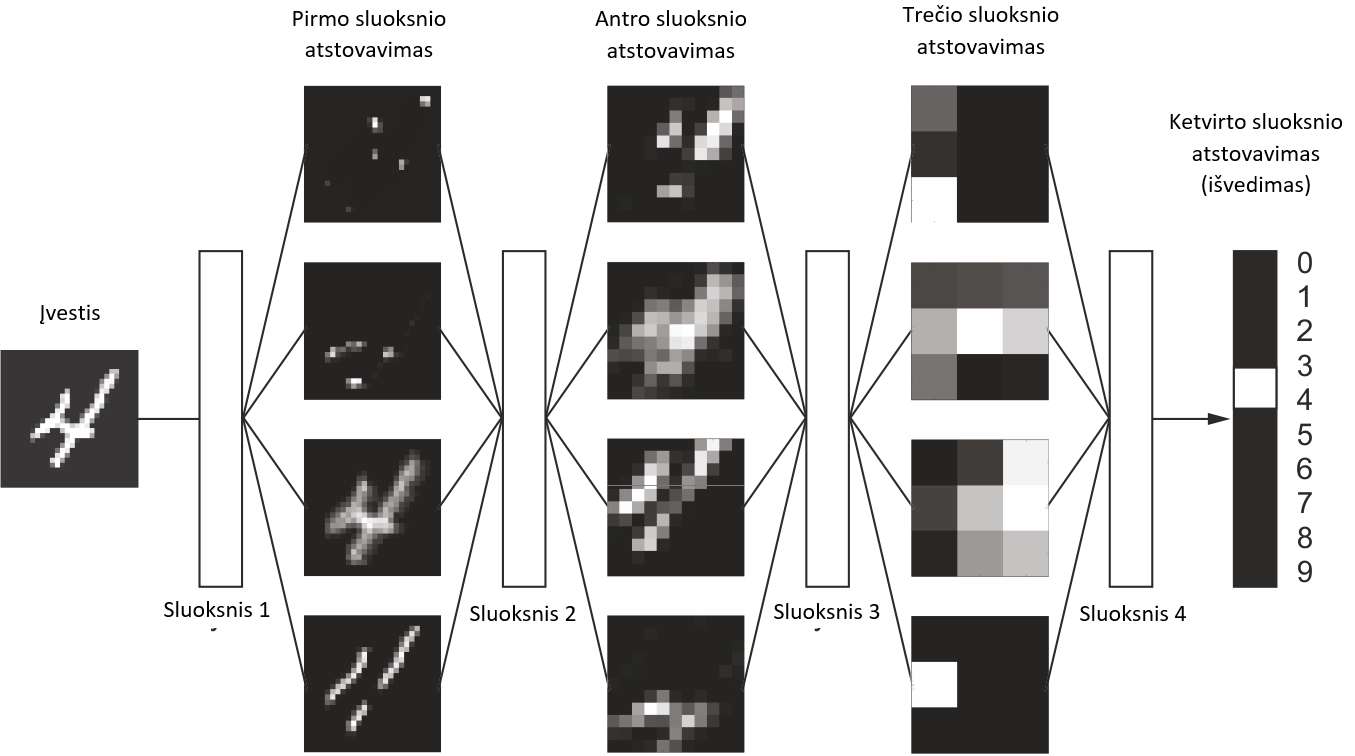
\includegraphics[scale=1.0]{img/figure_1-6}
  \caption{Gilios reprezentacijos, įgytos pagal skaitmenų klasifikacijos modelį.}
  \label{fig:DeepLearningDigit2}
\end{figure}

Apie gilų tinklą galima galvoti kaip apie daugiapakopę informacijos filtravimo operaciją, kurioje informacija pereina per filtrus ir yra „išvaloma“.

Specifiškai ką sluoksnis daro su galutiniais duomenimis yra laikoma sluoksnio svoryje. Galima pasakyti, kad sluoksnio įgyvendinta transformacija yra parametrizuojama pagal jo svorius kaip \ref{fig:NeuralNetwork} paveikslėlyje. Mokymas reiškia surasti tokias reikšmes kiekvieno sluoksnio svoriams, kad tinklas tinkamai pažymėtų įvedimą į jam priskirtą tikslą. Sudėtingumas yra tas, kad gilus neuroninis tinklas gali turėti daugybę parametrų, o keičiant vieną iš jų, bus paveikta visų kitų elgsena.

\begin{figure}[h!]
\centering
  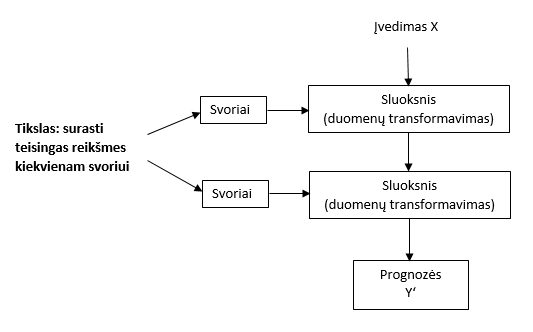
\includegraphics[scale=0.9]{img/figure_1-7}
  \caption{Neuroninis tinklas yra parametrizuojamas pagal svorius.}
  \label{fig:NeuralNetwork}
\end{figure}

\newpage

Kad kontroliuotume neuroninio tinko išvedimą, reikia mokėt apskaičiuoti kaip toli išvedimas buvo nuo laukiamo rezultato. Tai atlieka nuostolių funkcija (Loss function, pav. \ref{fig:NeuralNetwork2}). Nuostolių funkcija atsižvelgia į tinklo prognozes ir norimą tikslą, ir apskaičiuoja skirtumo balą, užfiksuodama kaip gerai tinklas atliko savo darbą.

\begin{figure}[h!]
\centering
  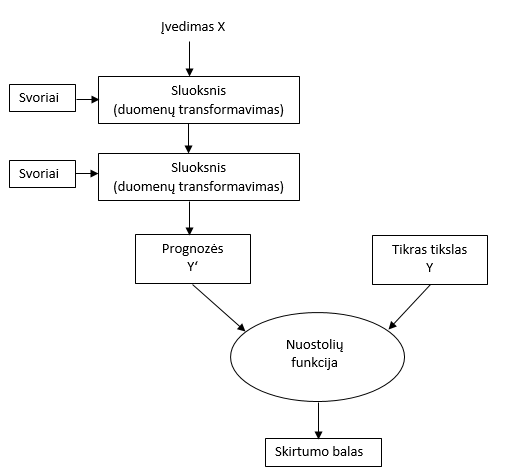
\includegraphics[scale=0.9]{img/figure_1-8}
  \caption{Nuostolių funkcija nustato tinklo išvedimo kokybę.}
  \label{fig:NeuralNetwork2}
\end{figure}

Giliojo mokymosi pagrindinis triukas yra naudoti šį balą kaip atsako signalą, kad šiek tiek pakoreguoti svorių vertę (Pav. \ref{fig:NeuralNetwork3}), tokiu būdu mažinant dabartinio pavyzdžio nuostolių balą. Šis koregavimas yra optimizatoriaus, kuris įgyvendina „skleidimo atgal“ („\textit{Backpropagation}“) algoritmą: pagrindinį giliojo mokymosi algoritmą, darbas.

\begin{figure}[h!]
\centering
  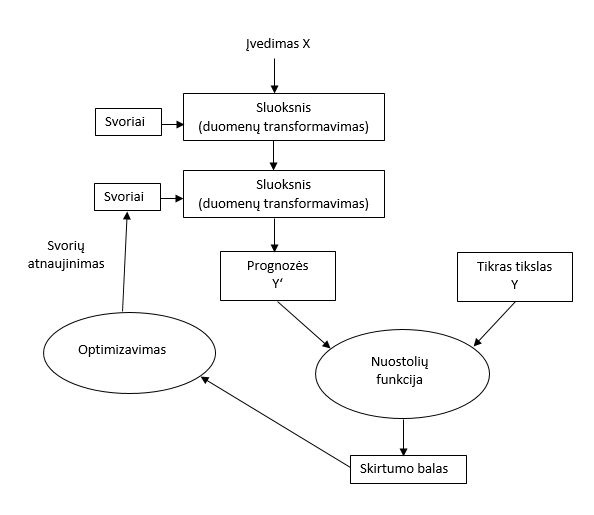
\includegraphics[scale=0.9]{img/figure_1-9}
  \caption{Skirtumo balas nusako kaip reikia keisti svorius.}
  \label{fig:NeuralNetwork3}
\end{figure}


Iš pradžių tinklo svoriams yra priskiriamos atsitiktinės vertės, todėl tinklas tiesiog įgyvendina porą atsitiktinių transformacijų. Aišku, kad pirmas išvedimas bus toli nuo to, ko mes norime ir nuostolių balas bus didelis. Bet su kiekvienu pavyzdžiu, kurį tinklas apdoroja, svoriai bus šiek tiek koreguojami ir nuostolių balas mažės. Tai bus kartojama reikiama kiekį kartų ir galiausiai gausime svorių vertes, su kuriomis nuostolių funkcija bus mažiausia. Tinklas su minimaliu nuostoliu yra tas, kurio rezultatai yra arčiausiai norimo tikslo. \cite{1}

\vspace{10mm}

Gilusis mokymasis pasiekė:
\begin{itemize}
  \item žmogaus gebėjimo lygio vaizdo klasifikacijos;
  \item žmogaus lygio kalbos atpažinimo;
  \item žmogaus lygio rankraščio transkripcijos;
  \item pagerintos konversijos iš teksto į kalbą;
  \item žmogaus lygio automatino vairavimo;
  \item patobulinto skelbimų taikymo, kurį naudoja „Google“, „Baidu“ ir „Bing“;
  \item geresnių paieškos rezultatų žiniatinklyje;
  \item gebėjimo atsakyti į natūralios kalbos klausimus;
\end{itemize}


\newpage

\section{\textit{Keras}}
\vspace{10mm}

Šiame skyriuje konstruosime neuroninį tinklą, kuris atpažins \textit{„Lego“} detales, su \textit{Keras} pagalba. Iš pradžių normalizuosime duomenų rinkinį, kuris yra sudarytas iš 6000 \textit{„Lego“} detalių paveikslėlių. Tam naudosime \textit{ImageJ} vaizdo apdorojimo programą. Toliau konstruosime tinklą. Tinklo konstravimui naudosime skirtingas architektūras, sudarytas iš skirtingų sluoksnių tipų, kurias palyginsime ir išsirinksime efektyviausią.

\subsection{Duomenų rinkinys}

\begin{enumerate} 

    \item Tinklo apmokymui naudosime $28\times28$ dydžio paveikslėlius. Visą duomenų rinkinį padalinsime į mokymo ir validavimo dalis. Mokymui skirsime 70\%, o validavimui -- 30\%.
    
    Prieš apmokant neuroninį tinklą normalizuosime visus mokymo duomenis. Iš pradžių konvertuosime pradinį apmokymo paveikslėlį (Pav. \ref{fig:Lego_Train_1}) iš RGB į pilkos spalvos (\textit{Grayscale}) ir pakeisime dydį į $100\times100$ (Pav. \ref{fig:Lego_Train_2}).
    
    \begin{figure}[h!]
    \centering
      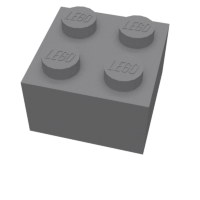
\includegraphics[scale=0.8]{img/lego_train_1}
      \caption{Nenormalizuotas paveikslėlis.}
      \label{fig:Lego_Train_1}
    \end{figure}

    \begin{figure}[h!]
    \centering
      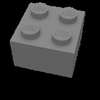
\includegraphics[scale=1.3]{img/lego_train_2}
      \caption{Pilkos spalvos, $100\times100$ apmokymo paveikslėlis.}
      \label{fig:Lego_Train_2}
    \end{figure}
    
    \newpage
    Taip pat turime normalizuoti testavimo duomenis. Pradžioje iš pradinio paveikslėlio (Pav. \ref{fig:Lego_Test_1}) pašalinsime foną (Pav. \ref{fig:Lego_Test_2}). Tada taip pat konvertuosime iš RGB į pilkos spalvos atspalvius (\textit{Grayscale}) ir pakeisime dydį į $100\times100$ (Pav. \ref{fig:Lego_Test_3}).
    
    \vspace{10mm}
    \begin{figure}[h!]
    \centering
      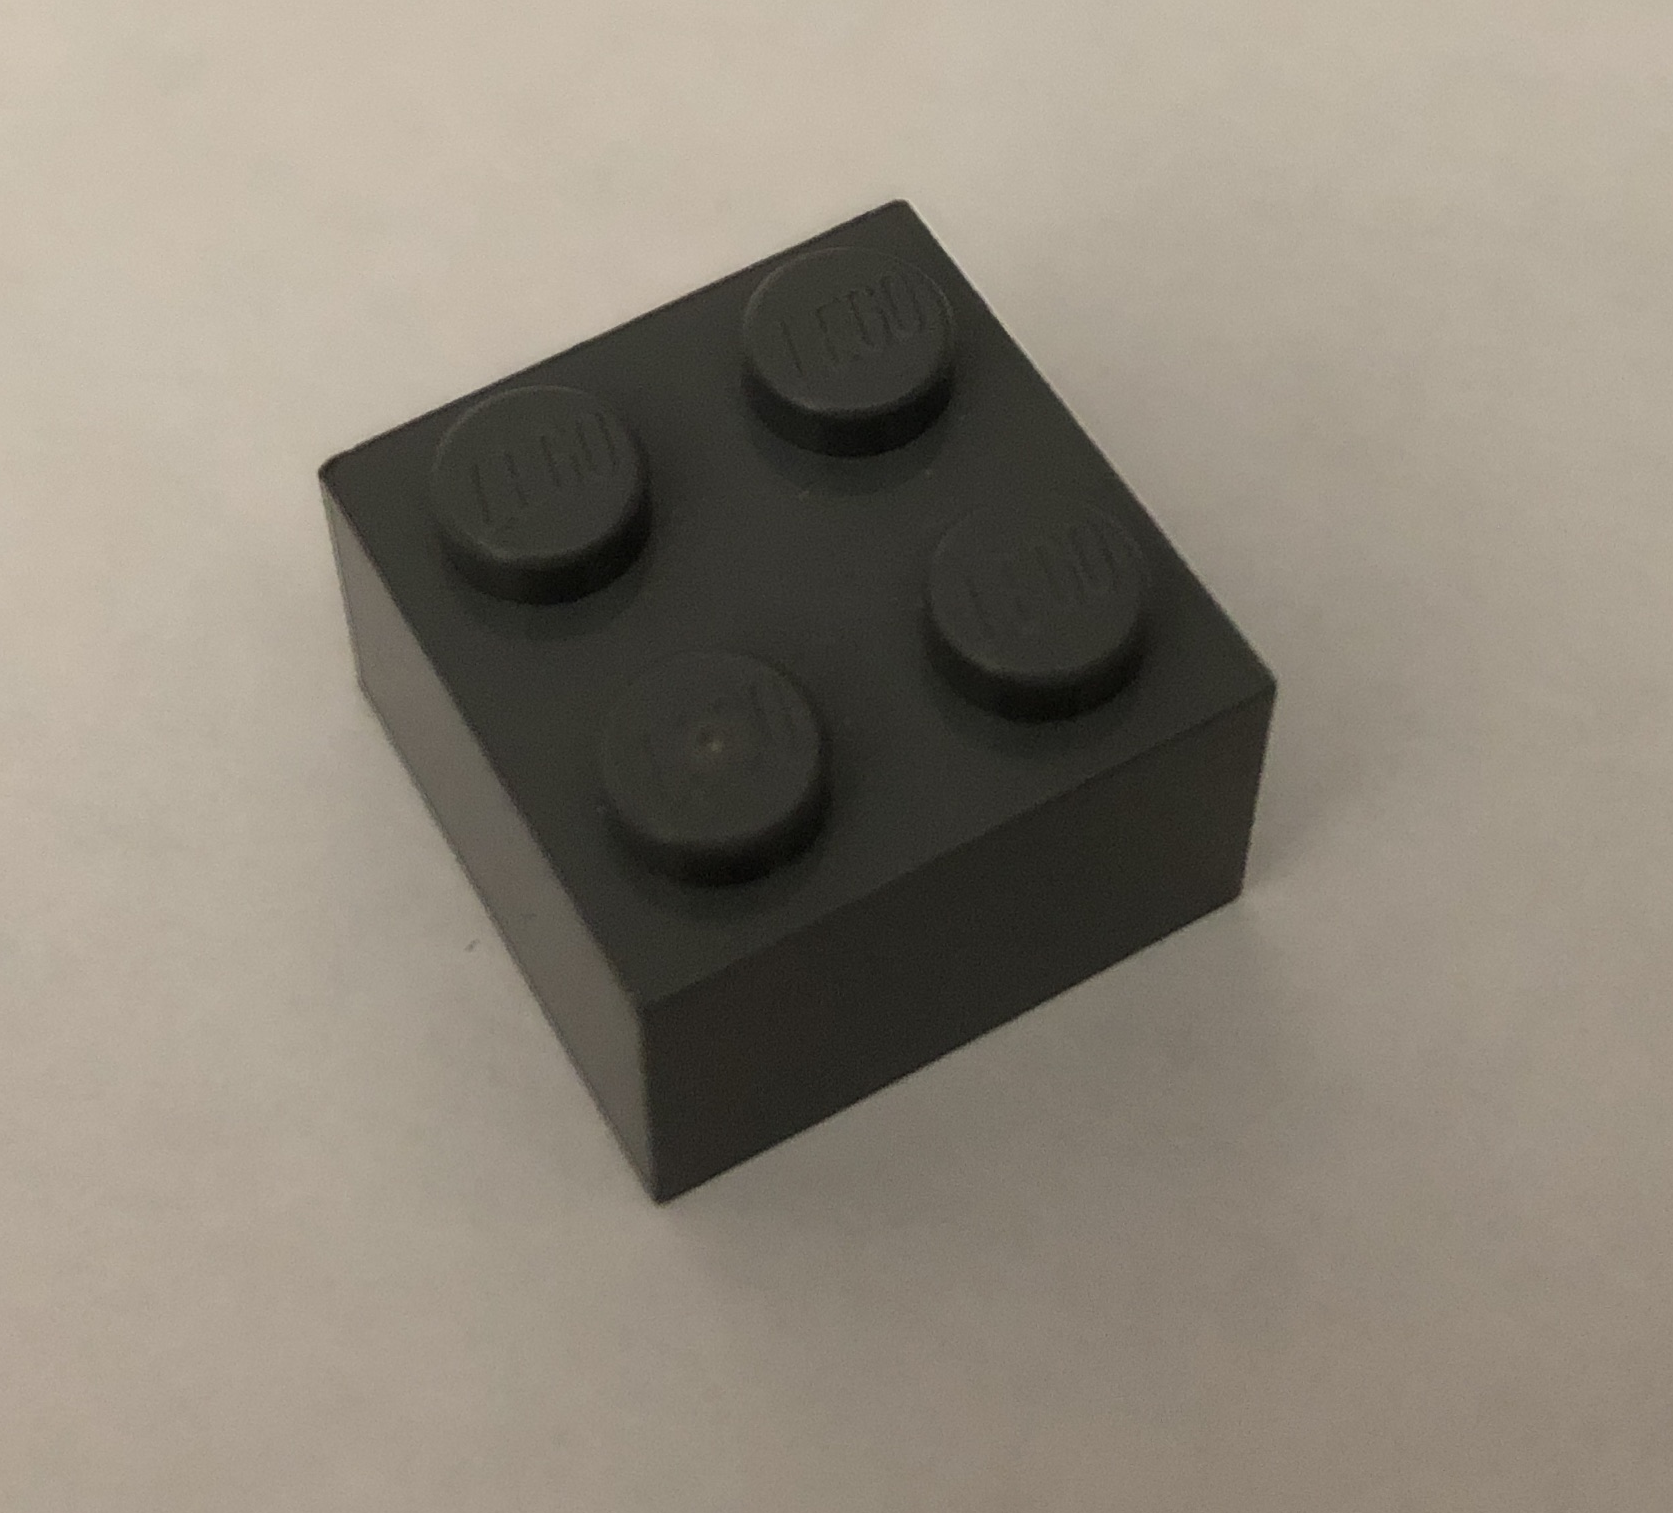
\includegraphics[scale=0.15]{img/lego_test_1}
      \caption{Testavimo paveikslėlis.}
      \label{fig:Lego_Test_1}
    \end{figure}
    
    \begin{figure}[h!]
    \centering
      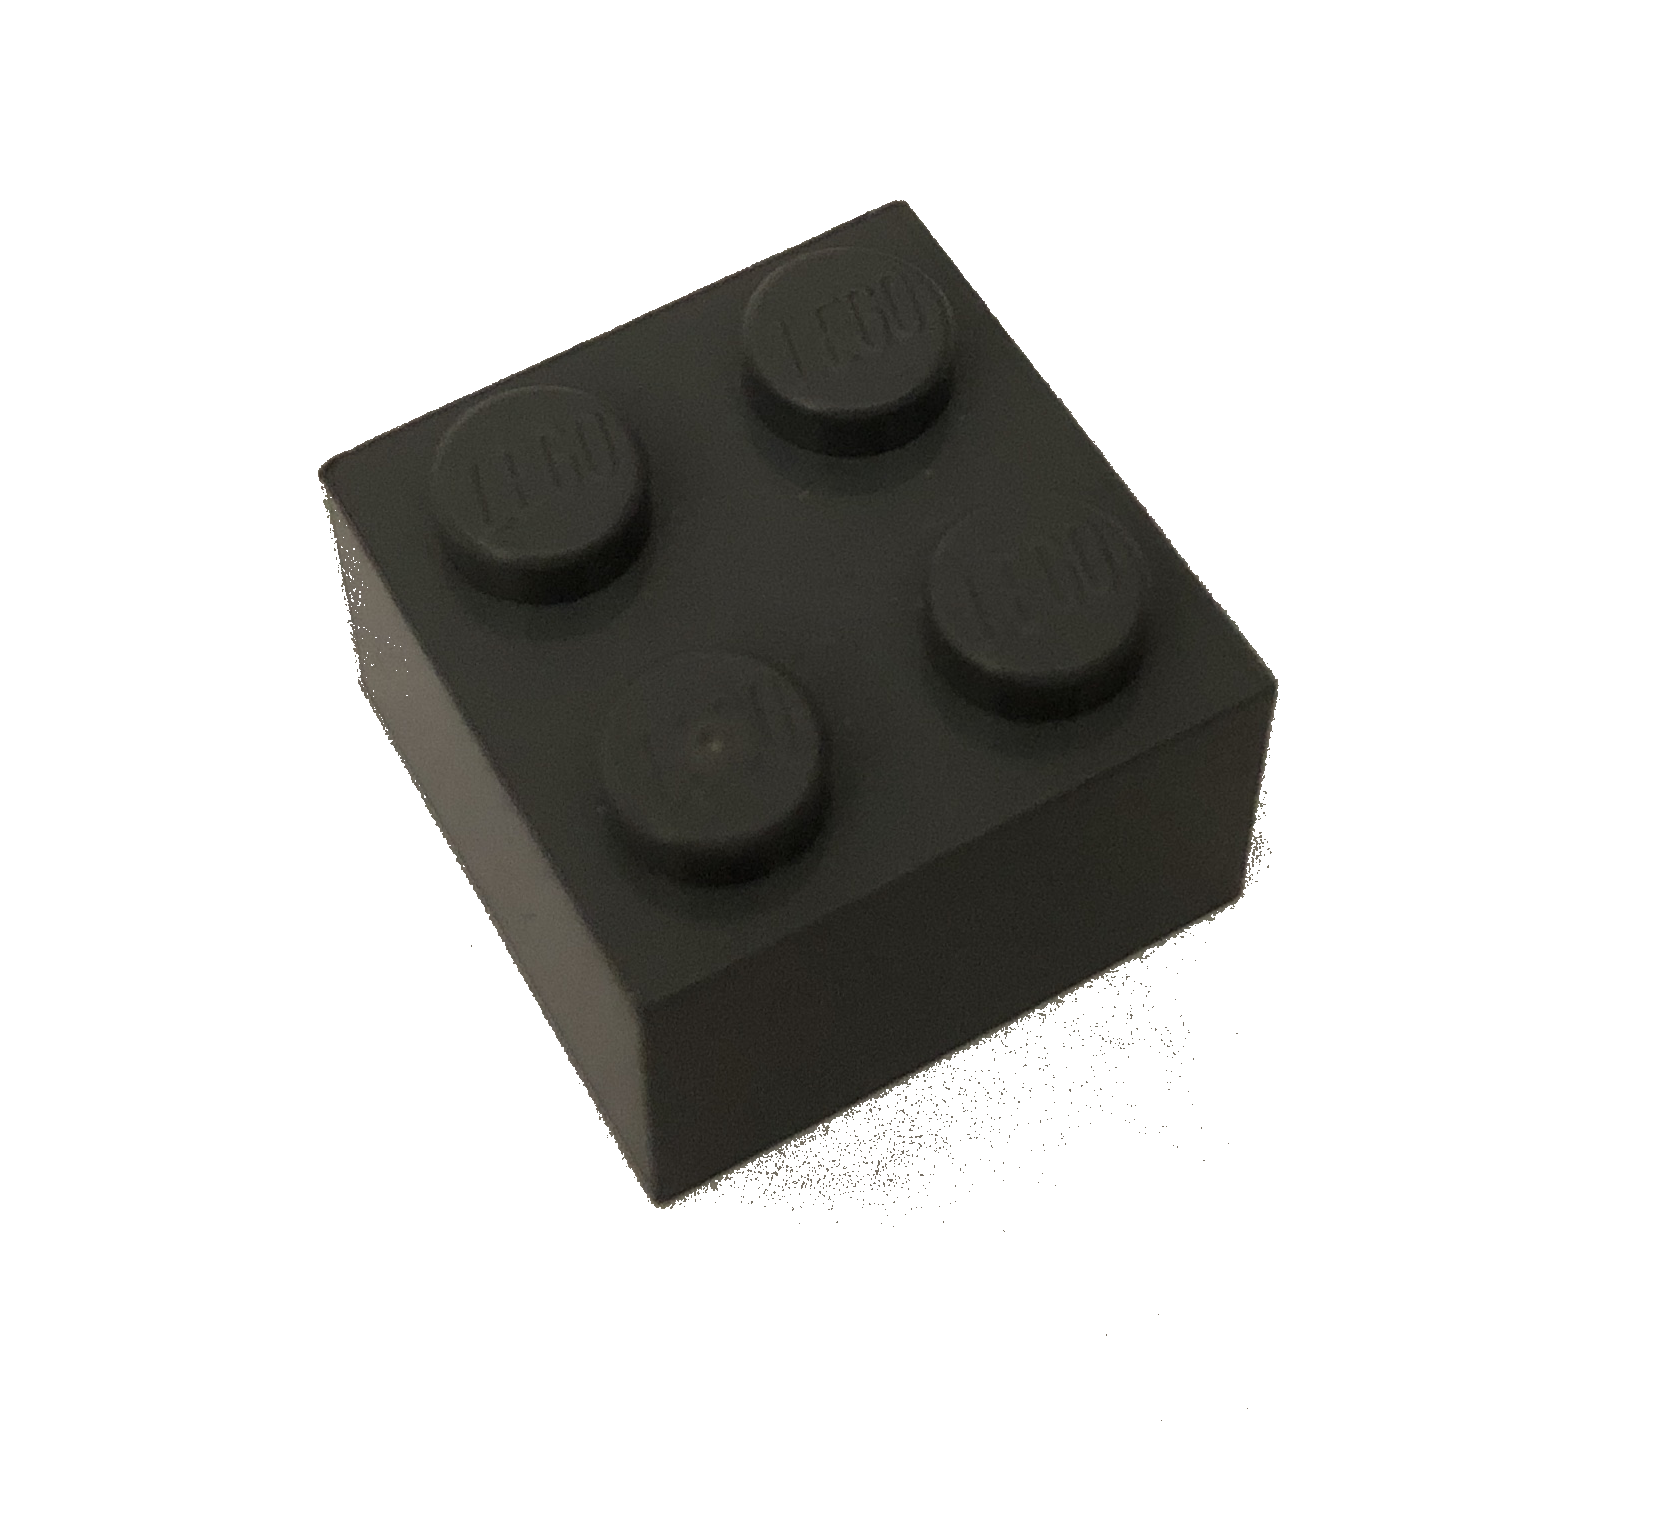
\includegraphics[scale=0.1]{img/lego_test_2}
      \caption{Testavimo paveikslėlis be fono.}
      \label{fig:Lego_Test_2}
    \end{figure}
    
    \begin{figure}[h!]
    \centering
      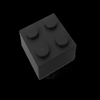
\includegraphics[scale=1.3]{img/lego_test_3}
      \caption{Pilkos spalvos, $100\times100$ testavimo paveikslėlis.}
      \label{fig:Lego_Test_3}
    \end{figure}
    
    \newpage
    \item Panaudosime \textit{ImageJ} metodą „Padidinti kontrastą“. Gavome tokius paveiklėlius:
    
    \vspace{10mm}
    \begin{figure}[h!]
    \centering
      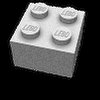
\includegraphics[scale=1.3]{img/lego_train_3}
      \caption{Apmokymo paveikslėlis.}
      \label{fig:Lego_Train_3}
    \end{figure}
    
    \begin{figure}[h!]
    \centering
      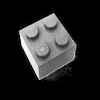
\includegraphics[scale=1.3]{img/lego_test_4}
      \caption{Testavimo paveikslėlis.}
      \label{fig:Lego_Test_4}
    \end{figure}
    
    \newpage
    \item Prieš normalizavimą, paveikslėlių histogramos atrodė taip:
    
    \begin{figure}[h!]
    \centering
      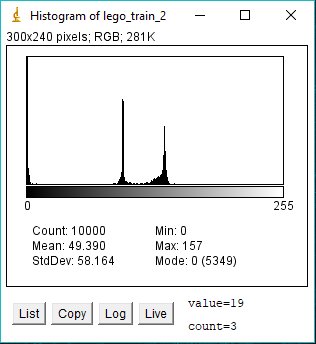
\includegraphics[scale=1.0]{img/histogram_train_1}
      \caption{Nenormalizuoto apmokymo paveikslėlio histograma.}
      \label{fig:histogram_train_1}
    \end{figure}
    
    \begin{figure}[h!]
    \centering
      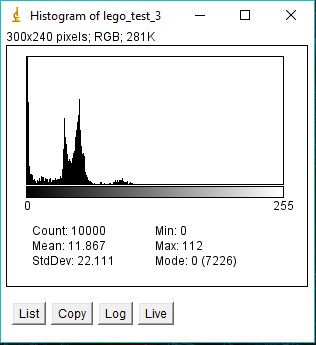
\includegraphics[scale=1.0]{img/histogram_test_1}
      \caption{Nenormalizuoto testavimo paveikslėlio histograma.}
      \label{fig:histogram_test_1}
    \end{figure}
    
    \newpage
    Po normalizavimo gavome tokias histogramas:
    
    \begin{figure}[h!]
    \centering
      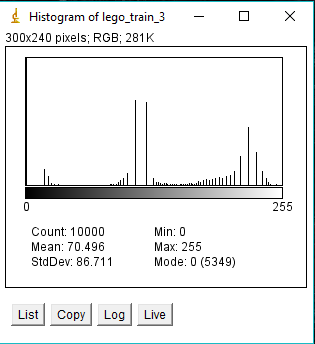
\includegraphics[scale=1.0]{img/histogram_train_2}
      \caption{Normalizuoto apmokymo paveikslėlio histograma.}
      \label{fig:histogram_train_2}
    \end{figure}
    
    \begin{figure}[h!]
    \centering
      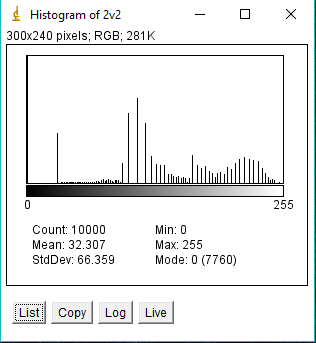
\includegraphics[scale=1.0]{img/histogram_test_2}
      \caption{Normalizuoto testavimo paveikslėlio histograma.}
      \label{fig:histogram_test_2}
    \end{figure}
    
    Matome, kad po normalizavimo histogramos tapo panašesnės.

    \newpage
    \item Panaudodami parašytą \textit{ImageJ} įskiepį (\textit{plugin}), centruosime duomenis. 
    
    \begin{figure}[h!]
    \centering
      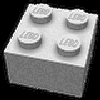
\includegraphics[scale=1.0]{img/train4}
      \caption{Centruotas apmokymo paveikslėlis.}
      \label{fig:train4}
    \end{figure}
    
    \begin{figure}[h!]
    \centering
      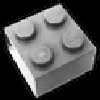
\includegraphics[scale=1.0]{img/test4}
      \caption{Centruotas testavimo paveikslėlis.}
      \label{fig:test4}
    \end{figure}
    
    
    \item Pritaikysime paveikslėliams \textit{ImageJ} Gauso filtrą.
    
    \begin{figure}[h!]
    \centering
      
\includegraphics[scale=1.0]{img/train5}
      \caption{Centruotas apmokymo paveikslėlis su Gauso filtru.}
      \label{fig:train5}
    \end{figure}
    
    \begin{figure}[h!]
    \centering
      
\includegraphics[scale=1.0]{img/test5}
      \caption{Centruotas testavimo paveikslėlis su Gauso filtru.}
      \label{fig:test5}
    \end{figure}
    
    \newpage
    \item Pakeisime paveikslėlių dydžius į $28\times28$. Taip pat panaudosime \textit{ImageJ} funkciją „Rasti kraštus“.
    
    \begin{figure}[h!]
    \centering
      
\includegraphics[scale=2.0]{img/train7}
      \caption{Apmokymo paveikslėlis dydžio $28\times28$ po funkcijos „Rasti kraštus“ panaudojimo.}
      \label{fig:train7}
    \end{figure}
    
    \begin{figure}[h!]
    \centering
      
\includegraphics[scale=2.0]{img/test7}
      \caption{Testavimo paveikslėlis dydžio $28\times28$ po funkcijos „Rasti kraštus“ panaudojimo.}
      \label{fig:test7}
    \end{figure}
    
    

\end{enumerate}

\newpage

\subsection{Modelis}

Prieš konstruojant neuroninį tinklą, apžiūrėkime sluoksnių tipus.

\subsubsection{Sluoksniai}

Mūsų modelyje naudosime \cite{3}:

\begin{itemize}
  \item Sąsūkos sluoksnis (\textit{Convolutional layer}) -- Sluoksnis, kuris uždeda filtrą (mūsų atveju $3\times3$) ir taip iš paveikslėlio yra išgaunami $3\times3$ dydžio sritys, su poslinkiu 1. (\ref{fig:conv2d} pav.) 
  \item Didžiausio atmetimo sluoksnis (\textit{Max-Pool layer}) -- Sluoksnis, kuris sumažina paveikslėlio reprezentaciją dvigubai (naudojamas $2\times2$ filtras). (\ref{fig:maxpool2d} pav.) 
  \item Tirštasis sluoksnis (\textit{Dense layer}) -- Sluoksnis, kuris jungia visus neuronus iš praeito sluoksnio, su visais šio sluoksnio neuronais.
  \item Atmetimo sluoksnis (\textit{Dropout layer}) -- dalis neuronų yra ignoruojama, kad išvengtume permokymo (\textit{overfitting}).
\end{itemize} 


\begin{figure}[h!]
\centering
  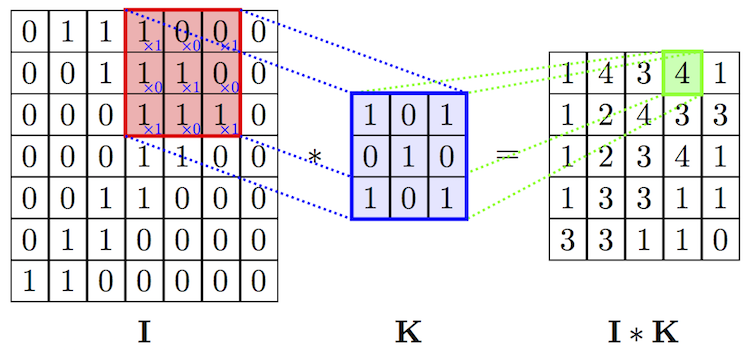
\includegraphics[scale=1.3]{img/conv2d}
  \caption{Sąsūkos sluoksnis.}
  \label{fig:conv2d}
\end{figure}


\begin{figure}[h!]
\centering
  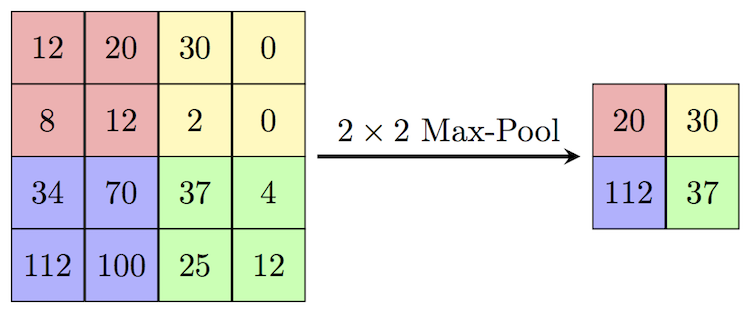
\includegraphics[scale=1.3]{img/maxpool2d}
  \caption{Didžiausio atmetimo sluoksnis.}
  \label{fig:maxpool2d}
\end{figure}



\newpage

\subsubsection{Architektūra}

\begin{enumerate}
    \item Iš pradžių sukonstruosim tinklą su vienu tirštuoju sluoksniu, kuris turės 64 neuronus. Mokymas vyks 40 iteracijų.
      
    \begin{figure}[h!]
    \centering
    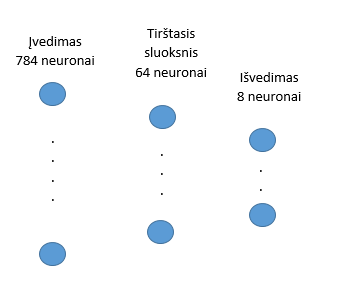
\includegraphics[scale=0.8]{img/tinklas1}
    \caption{Pirmas tinklas.}
    \label{fig:tinklas1}
    \end{figure}
    
    Toks tinklas pasiekė tik 18.0\% atpažinimo tikimybę.
      
    \begin{figure}[h!]
    \centering
    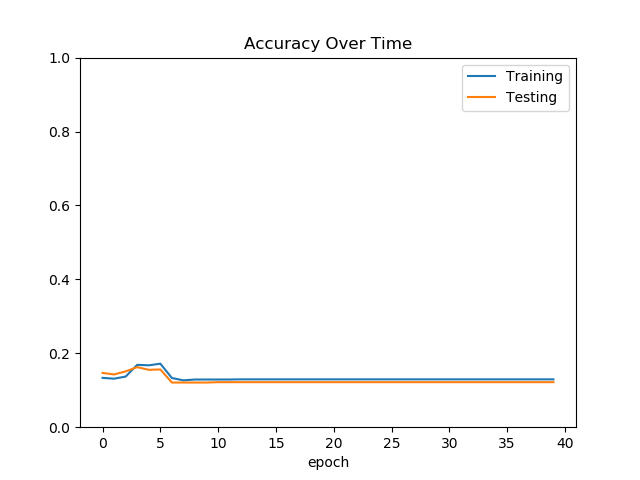
\includegraphics[scale=0.6]{img/grafas1}
    \caption{Pirmo tinklo grafas.}
    \label{fig:grafas1}
    \end{figure}


    \newpage
    
    
    
    \item Naujas tinklas turės du tirštuosius sluoksnius po 128 neuronus. Mokymas vyks 40 iteracijų.
    
    \begin{figure}[h!]
    \centering
    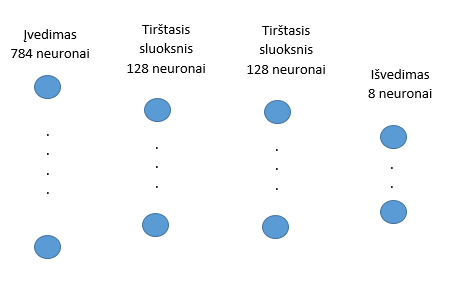
\includegraphics[scale=0.8]{img/tinklas2}
    \caption{Antras tinklas.}
    \label{fig:tinklas2}
    \end{figure}
    
    Toks tinklas pasiekė 22.44\% atpažinimo tikimybę.
    
    \begin{figure}[h!]
    \centering
    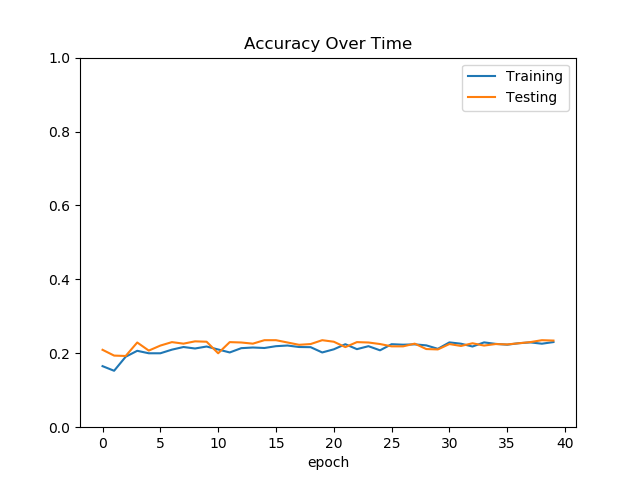
\includegraphics[scale=0.6]{img/grafas2}
    \caption{Antro tinklo grafas.}
    \label{fig:grafas2}
    \end{figure}
    
    
    \newpage
    
    \item Prieš tirštuosius sluoksnius įdėsim vieną sąsūkos sluoksnį, kuris turės 32 filtrus, ir išgaus iš paveikslėlio $3\times3$ dydžio sritys, su poslinkiu 1. Po sąsūkos sluoksnio bus didžiausio atmetimo sluoksnis ($2\times2$ filtras). Mokymas vyks 40 iteracijų.
    
    
    \begin{figure}[h!]
    \centering
    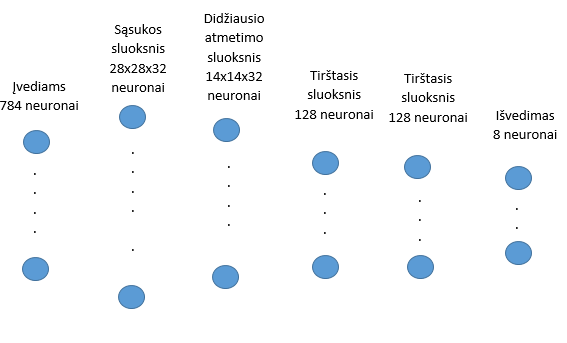
\includegraphics[scale=0.8]{img/tinklas3}
    \caption{Trečias tinklas.}
    \label{fig:tinklas3}
    \end{figure}
    
    
    Toks tinklas pasiekė 79.4\% atpažinimo tikimybę.
    
    
    \begin{figure}[h!]
    \centering
    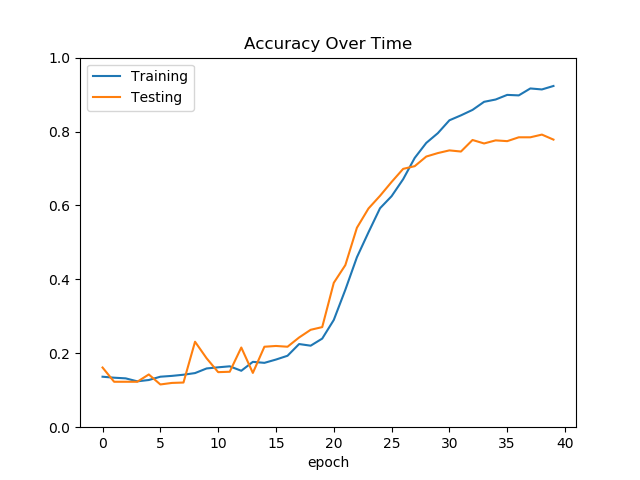
\includegraphics[scale=0.6]{img/grafas3}
    \caption{Trečio tinklo grafas.}
    \label{fig:grafas3}
    \end{figure}
    
    
    
    \newpage
    
    \item Kad išvengtume permokymo, tarp tirštųjų sluoksnių įdėsim atmetimo sluoksnį su koeficientu 0.5.
    
    
    \begin{figure}[h!]
    \centering
    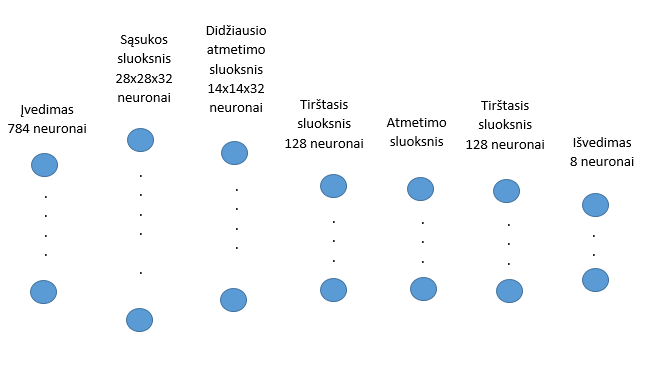
\includegraphics[scale=0.8]{img/tinklas4}
    \caption{Ketvirtas tinklas.}
    \label{fig:tinklas4}
    \end{figure}
    
    
    Toks tinklas pasiekė 77.81\% atpažinimo tikimybę.
    
    
    \begin{figure}[h!]
    \centering
    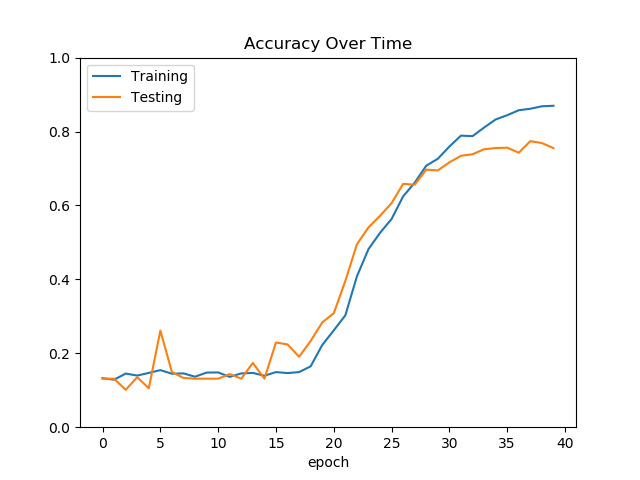
\includegraphics[scale=0.6]{img/grafas4}
    \caption{Ketvirto tinklo grafas.}
    \label{fig:grafas4}
    \end{figure}
    
    \newpage
    
    \item Patikrinkime, kaip keičiasi tinklo atpažinimas pakeitus tirštųjų sluoksnių neuronų skaičių.
    
    \begin{figure}[h!]
    \centering
    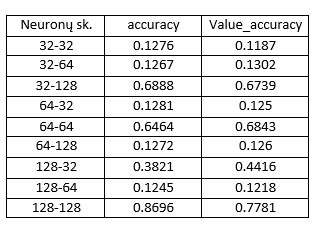
\includegraphics[scale=0.9]{img/DenseLayerTable}
    \caption{Tirštųjų sluoksnių neuronų sk. lentelė.}
    \label{fig:DenseTable}
    \end{figure}
    
    
    \begin{figure}[h!]
    \centering
    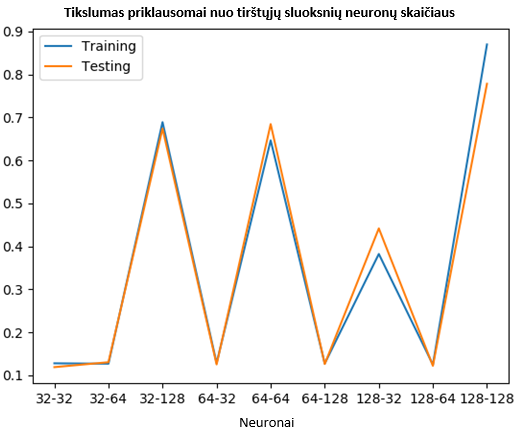
\includegraphics[scale=0.9]{img/DenseLayerGraph}
    \caption{Tirštųjų sluoksnių neuronų sk. grafas.}
    \label{fig:DenseGraph}
    \end{figure}

\end{enumerate}

Kaip matome didžiausią atpažinimo tikimybę tinklas pasiekė, kai jis buvo sudarytas iš vieno sąsūkos sluoksnio, kuris turi 32 filtrus ir išgauna iš paveikslėlio $3\times3$ dydžio sritis, su poslinkiu 1. Po sąsūkos sluoksnio eina didžiausio atmetimo sluoksnis ($2\times2$  filtras). Tada eina 2 tirštieji sluoksniai (turintys po 128 neuronus), tarp kurių yra atmetimo sluoksnis su koeficientu 0.5.

\newpage

\section{\textit{TensorFlow.js}}
\vspace{10mm}

Vis daugiau kūrėjų naudoja \textit{Keras} ir \textit{TensorFlow} savo giliojo mokymosi projektuose. Viena didžiausių kliūčių žmonėms, kurie nori išbandyti gilųjį mokymą, yra visas reikalingos įrangos nustatymas, kuris gali užimti nemažai laiko. \textit{TensorFlow.js} neturi tokio trūkumo, nes tinklą, apmokytą naudojant \textit{TensorFlow.js}, galima paleisti tiesiogiai per naršyklę naudojant \textit{JavaScript}.\cite{12}

\subsection{Istorija}

Prieš rašant apie \textit{TensorFlow.js}, reikėtų papasakoti apie patį \textit{TensorFlow}. \textit{TensorFlow} buvo sukurtas 2011 m. \textit{„Google“}, kaip mašininio mokymosi/gilaus mokymosi programų biblioteka. \textit{TensorFlow} yra parašytas naudojant \textit{C++}, kuris leidžia dirbti žemam lygyje. \textit{TensorFlow} turi ryšį su kitom kalbom, pvz., \textit{Python}, \textit{R} ir \textit{Java}.  Taigi, akivaizdus klausimas: kas gi apie \textit{JavaScript}? Tradiciškai, \textit{JavaScript}, gilusis mokymasis buvo atliekamas naudojant API. API buvo sukurtas naudojant tam tikrą karkasą, o modelis buvo įdiegtas serveryje. Klientas siuntė užklausą naudodamas \textit{JavaScript}, kad gauti rezultatus iš serverio. 
\par
2017 m. pasirodė projektas vadinamas \textit{Deeplearn.js}, kurio tikslas -- leisti gilųjį mokymą atlikti \textit{JavaScript} be API vargo. Tačiau buvo klausimų apie greitį. \textit{DeepLearn.js} kodas negalėjo būti leidžiamas ant GPU. Kad išspręsti šią problemą, buvo pritaikytos \textit{WebGL} (\textit{JavaScript} API, skirta interaktyviosios 2D ir 3D grafikos vaizdavimui bet kurioje suderinamoje interneto naršyklėje, nenaudojant papildinių) galimybes \textit{DeepLearn.js}, taip gimė \textit{TensorFlow.js}. \cite{12}

\subsection{\textit{TensorFlow.js} naudojimas}

Ką galima daryti su \textit{TensorFlow.js}?

\begin{itemize}
  \item Galima importuoti esamą, iš anksto parengtą modelį. Jei turime  \textit{TensorFlow}, arba \textit{Keras} modelį, kuris buvo anksčiau apmokytas, galime jį išsaugoti plačiai žinomu \textit{Json} (\textit{JavaScript Object Notation}) formatu, po to konvertuoti jį į \textit{TensorFlow.js} formatą ir įkelti į naršyklę, kad galėtumėme daryti išvadas.
  \item Galima iš naujo apmokyti importuotą modelį. Galime naudoti perkėlimo mokymą, kad patobulinti esamą modelį, naudojant nedidelį kiekį duomenų, surinktų naršyklėje, naudojant techniką, vadinamą \textit{„Image Retraining“}.
  \item Taip pat galima naudoti \textit{TensorFlow.js}, norėdami apibrėžti, mokyti ir paleisti modelius visiškai naršyklėje naudojant \textit{Javascript} ir aukšto lygio sluoksnių API (\textit{LayerAPI}). Aukšto lygio sluoksnių API yra labai panašus į \textit{Keras} API.
\end{itemize} 

\textit{Tensorflow.js} suteikia\cite{12}:

\begin{itemize}
  \item \textit{CoreAPI} -- susitvarko su žemo lygio kodu.
  \item \textit{LayerAPI} -- pastatytas ant \textit{CoreAPI} ir palengvina mūsų gyvenimą, padidinant abstrakcijos lygį.
\end{itemize} 

\subsection{\textit{CoreAPI}}

\textit{TensorFlow.js} yra biblioteka, leidžianti nustatyti ir paleisti skaičiavimus naudojant \textit{JavaScript} tenzorius. Tenzorius yra vektorių ir matricų apibendrinimas į aukštesnes  dimensijas. 
\par
\textit{TensorFlow.js} centrinis duomenų vienetas yra \textit{tf.Tensor}: reikšmių rinkinys, suformuotas į masyvą, kurio dimensija yra vienas, arba daugiau. \textit{tf.Tensors} yra labai panašūs į daugiamatį masyvą.\cite{9}
\par
\textit{tf.Tensor} taip pat turi šias savybes:

\begin{itemize}
  \item \textit{rank}: nustato, kiek matmenų yra tenzoriuje.
  \item \textit{shape}: apibrėžia duomenų matmenį.
  \item \textit{dtype}: kuris apibrėžia tenzoriaus duomenų tipą.
\end{itemize} 

\begin{figure}[h!]
\centering
  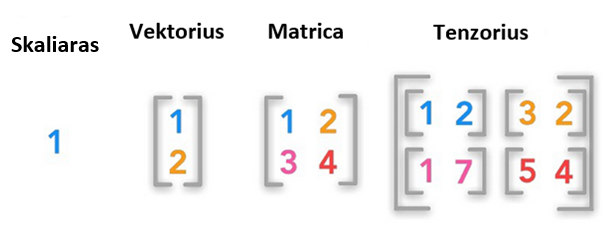
\includegraphics[scale=0.7]{img/Tensor.PNG}
  \caption{Skaliaras, vektorius, matrica ir tenzorius.}
  \label{fig:tensor}
\end{figure}

\begin{itemize}
  \item Skaliaras yra vienas numeris. Pavyzdžiui, x = 1.
  \item Vektorius yra skaičių masyvas. Pavyzdžiui, x = [1,2].
  \item Matrica yra 2-D masyvas
([[1, 2],
  [3, 4],
  [5, 6]]).
  \item Tenzorius yra n-dimensijos masyvas su n > 2.
\end{itemize} 

\textit{TensorFlow.js} turi naudingų funkcijų įprastiems atvejams, pvz., \textit{„Scalar“}, \textit{„1D“}, \textit{„2D“}, \textit{„3D“} ir \textit{„4D“} tenzoriams, taip pat daug funkcijų, skirtų inicijuoti tenzorius giliojo mokymosi tikslais.

\subsubsection{Vaizdų aktyvavimų išsaugojimas ir įkėlimas.}

\textit{TensorFlow.js} yra pakankamai naujas projektas, todėl jis dar neturi viso reikalingo funkcionalumo. Vienas iš jų yra vaizdų aktyvavimų išsaugojimas/įkėlimas. Tai buvo reikalingas funkcionalumas mūsų projekte, todėl mums teko jį realizuoti patiems. Visi vaizdų aktyvavimai buvo saugomi kaip tenzoriai, todėl teko panaudoti \textit{TensorFlow.js} funkcijas skirtas darbui su tenzoriais.

Tenzoriai yra saugomi pavidalo [n, 1024], kur n yra vieno objekto paveikslėlių kiekis (Pav.\ref{fig:image_tensors1}).

\begin{figure}[h!]
\centering
  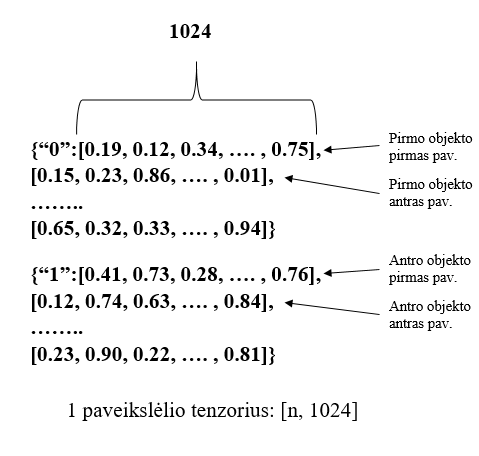
\includegraphics[scale=0.9]{img/pav_tensors1.PNG}
  \caption{Paveikslėlių aktyvavimų tenzoriai.}
  \label{fig:image_tensors1}
\end{figure}

Po išsaugojimo \textit{Json} (\textit{JavaScript Object Notation}) formatu, kiekvieno vaizdo tenzorius pasikeitė į pavidalą [1, n $\times$ 1024] (Pav.\ref{fig:image_tensors2}).

\begin{figure}[h!]
\centering
  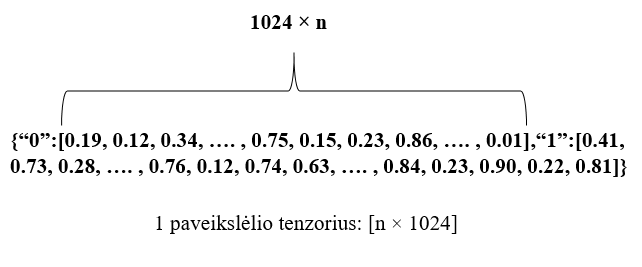
\includegraphics[scale=0.9]{img/pav_tensors2.PNG}
  \caption{Paveikslėlių aktyvavimų tenzoriai išsaugoti \textit{Json} formatu.}
  \label{fig:image_tensors2}
\end{figure}

Kad įkeltume išsaugotas paveikslėlių aktyvacijas į modelį, reikėjo kiekvieno objekto tenzorių padalinti iš 1024, kad gautume kiekvieno objekto paveikslėlių kiekį. Toliau panaudojant \textit{TensorFlow.js} tensor funkciją, sukurti kiekvieno paveikslėlio tenzorių.

\subsection{\textit{LayerAPI}}
\vspace{10mm}

Sluoksniai yra pagrindinis statybinis blokas gilaus mokymo modelio konstravimui. Kiekvienas jų paprastai atliks tam tikrą skaičiavimą, kad transformuotų savo įvestį į savo \textit{produkciją}. Po gaubtu kiekvienas sluoksnis naudoja \textit{Tensorflow.js} \textit{CoreAPI}.
\par
Sluoksniai automatiškai pasirūpins, kad būtų sukurti ir inicijuoti įvairūs vidiniai kintamieji/svoriai. Taigi, iš esmės jie palengvina gyvenimą, didindami abstrakcijos lygį.\cite{12}

\subsection{\textit{Handtrack.js}}

Darbui atlikti naudojome \textit{Handtrack.js} biblioteką, kuri, kaip galima suprasti iš pavadinimo, leidžia stebėti ir surasti rankų poziciją ant paveikslėlio. Ši biblioteka suranda ranką ant paveikslėlio ir apibrėžia  keturkampį aplink ją. Mūsų atveju reikėjo surasti ranką vaizde, kuris buvo filmuojamas realiu laiku. \textit{Handtrack.js} dalino vaizdo įrašą į atskirus kadrus ir surasdavo rankos poziciją kiekviename iš jų (Pav.\ref{fig:handtrack}).

\newpage

\begin{figure}[h!]
\centering
  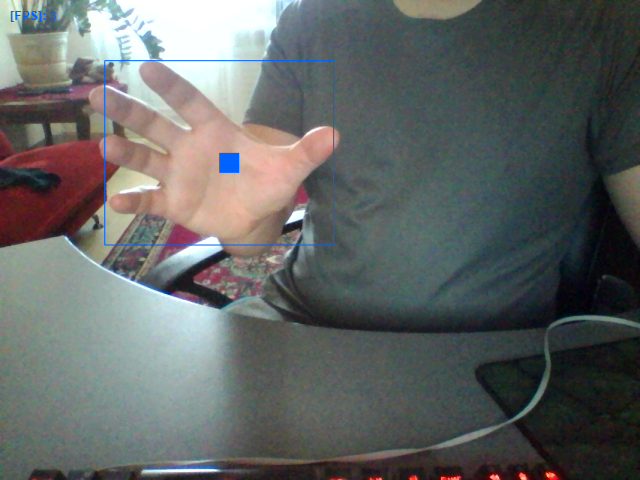
\includegraphics[scale=0.4]{img/handtrack.png}
  \caption{Rankos atpažinimas realiu laiku.}
  \label{fig:handtrack}
\end{figure}

\textit{Handtrack.js} gali būti naudojamas daugelyje atvejuose. Kai kurie iš jų\cite{11}:

\begin{itemize}
  \item Kai pelės judėjimas gali būti susietas su rankos judesiu kontrolės tikslais.
  \item Kai rankų judesiai gali rodyti reikšmingus signalus.
  \item Scenarijai, kuriuose žmogaus rankų judėjimas gali būti naudojamas veiklos atpažinimui.
\end{itemize}

\subsubsection{\textit{Handtrack.js} API}

Pateikiami keli metodai. Du pagrindiniai metodai yra  \textit{load()}, įkeliantis rankų aptikimo modelį ir \textit{detect()} metodas, skirtas gauti prognozes\cite{11}:

\begin{itemize}
  \item \textit{load()} -- priima pasirinktinius modelio parametrus, kurie leidžia valdyti modelio veikimą. Šis metodas įkelia iš anksto paruoštą rankų aptikimo modelį (Pav.\ref{fig:handtrack1}).
  \item \textit{detect()} -- priima įvedimo šaltinio parametrą (\textit{html} vaizdo objektą) ir grąžina apribojimo dėžutės, kurį nurodo rankos poziciją vaizde, dydį ir poziciją (Pav.\ref{fig:handtrack2}).
\end{itemize}

\begin{figure}[h!]
\centering
  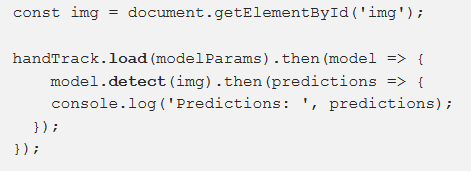
\includegraphics[scale=0.9]{img/handtrack1.PNG}
  \caption{\textit{Handtrack.js} \textit{load()} ir \textit{detect()} funkcijos.}
  \label{fig:handtrack1}
\end{figure}

\begin{figure}[h!]
\centering
  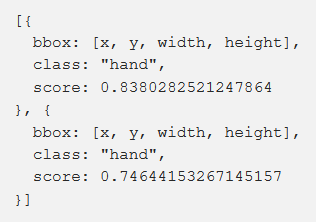
\includegraphics[scale=0.9]{img/handtrack2.PNG}
  \caption{Prognozavimo rezultatai.}
  \label{fig:handtrack2}
\end{figure}

\newpage

\subsubsection{Duomenų surinkimas ir apribojimai}

Apmokyti \textit{Handtrack.js} buvo naudojami 4800 rankų vaizdų skirtinguose aplinkose (patalpose, lauke). Duomenys buvo padalinti, skiriant 80\% apmokymui ir 20\% testavimui.\cite{11}
\par
Pastebėjome, kad kartais prognozės yra neteisingos (pvz. kartais veidas aptinkamas kaip ranka). Manaome, kad tai atsitinka dėl skirtingų kamerų ir skirtingo apšvietimo. Tai galima būtu patobulinti papildomais duomenimis.

\subsection{Mokymosi perkėlimas (\textit{Transfer learning})}

Sudėtingi gilaus mokymo modeliai gali turėti milijonus parametrų, o pats mokymas dažnai reikalauja didelių skaičiavimo išteklių, papildomai mokymas gali užimti daug laiko. Mokymosi perkėlimas yra technika, kuri sutrumpina visą tai, paimdama modelį, kuris jau yra apmokytas susijusioje užduotyje, ir pakartotinai panaudojant tą modelį. Mes galime pritaikyti esamas žinias iš anksto parengtame modelyje, kad nustatytumėme savo vaizdo klases, naudojant daug mažiau mokymo duomenų, nei reikalautų originalus modelis. Tai naudinga sparčiai plėtojant naujus modelius, taip pat pritaikant modelius išteklių ribotoje aplinkoje, pavyzdžiui, naršyklėse ir mobiliuosiuose įrenginiuose. Dažniausiai, atliekant perkėlimą, nekoreguojame pradinių modelio svorių. Vietoj to mes pašaliname galutinį sluoksnį ir apmokame naują modelį (Pav.\ref{fig:transfer_learning}). Savo darbui atlikti naudojome mokymosi perkėlimą, panaudojant \textit{MobileNet} modelį, kuris jau yra apmokytas atpažinti tūkstančius skirtingų objektų tipų iš paveikslėlių.\cite{9}

\begin{figure}[h!]
\centering
  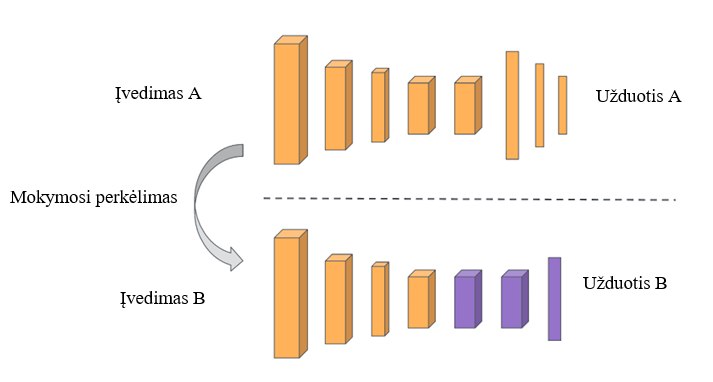
\includegraphics[scale=0.7]{img/TransferLearning.PNG}
  \caption{Mokymosi perkėlimas (\textit{Transfer learning}).}
  \label{fig:transfer_learning}
\end{figure}

\newpage

\subsubsection{Modelio konstravimas}

Pradžioje reikia įkelti \textit{MobileNet} modelį. Po to nustatyti kamerą, per kurią bus gaunamas vaizdas, pagal kurį bus atliekamas atpažinimas.

\begin{figure}[h!]
\centering
  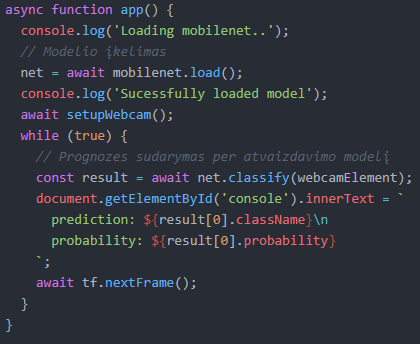
\includegraphics[scale=0.9]{img/Prog1.PNG}
  \caption{\textit{MobileNet} įkelimas.}
  \label{fig:Prog1}
\end{figure}

\newpage

Dabar padarysime šį tinklą naudingesnį. Prie modelio pridėsime 3 klasių objekto klasifikatorių, su kurio pagalba galima bus tinklą apmokyti atpažinti 3 skirtingus objektus. Naudosiu modelį vadinamą „K artimiausiu kaimynų klasifikatoriumi“ (\textit{K-Nearest Neighbors Classifier}), kuris leidžia kameros vaizdus (iš tikrųjų, jų \textit{MobileNet} aktyvavimus) sudėti į skirtingas kategorijas (arba klases), o kai vartotojas prašo daryti prognozę, mes paprasčiausiai pasirenkame klasę, turinčią labiausiai panašią aktyvavimą į tą, kurio atpažinimą darome.

\begin{figure}[h!]
\centering
  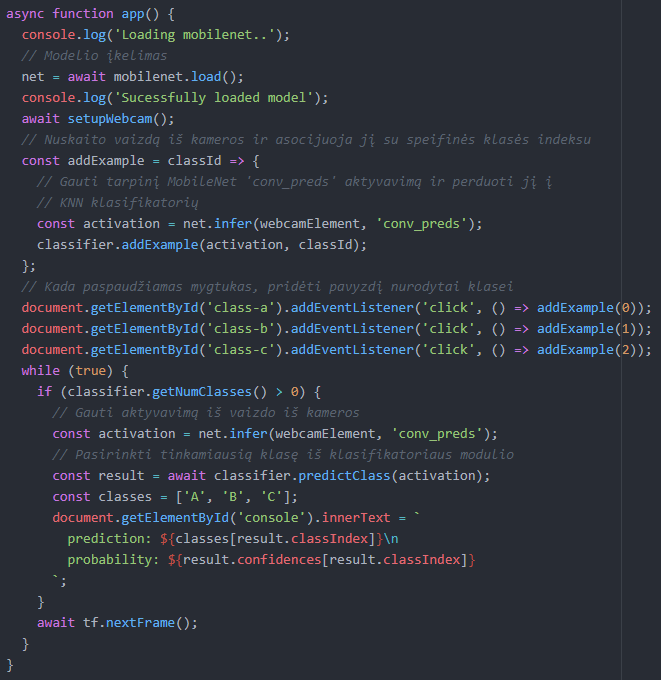
\includegraphics[scale=0.9]{img/Prog2.PNG}
  \caption{Modelio konstravimas.}
  \label{fig:Prog2}
\end{figure}

Toks tinklas atpažįsta rankoje laikomus didesnius, skirtingos spalvos objektus su tikimybe 79\%, o vienodos spalvos -- 74\%. Mažesnius, skirtingos spalvos objektus atpažįsta su tikimybe 76\%, o vienodos spalvos -- 68\%. Pridedant prie modelio papildomas klases atpažinti didesnį kiekį objektų, naršyklė negalėjo susitvarkyti su apmokytu tinklu. 

\subsection{\textit{MobileNet} modelis}

Mokymosi perkėlimui naudojome \textit{MobileNet} modelį, nes jo architektūra yra pakankamai lengva. Jis naudoja giliai atskiriamas sąsūkas (\textit{depthwise separable convolution}), kas iš esmės reiškia, kad kiekviename spalviniame kanale yra atliekama viena sąsūka, o ne visų trijų kanalų sujungimas ir išlyginimas (\textit{flatten}). Tai lemia įvesties kanalų filtravimą. \textit{MobileNet} gili sąsūka (\textit{depthwise convolution}) priskiria vieną filtrą kiekvienam įvesties kanalui (Pav.\ref{fig:depthwise_convolution}). Tada taškinė sąsūka (pointwise convolution) taiko 1x1 filtrą, kad sujungti išvedimą su gilią sąsūką (Pav.\ref{fig:pointwise_convolution}). Standartinė sąsūka filtruoja ir sujungia įvedimus į naują išvesties rinkinį vienu žingsniu (Pav.\ref{fig:standart_convolution}), o giliai atskiriama (depthwise separable convolution) tai padalija į du sluoksnius: atskirą filtravimo sluoksnį ir atskirą sluoksnį jungimui. Šis faktorizavimas labai efektyviai sumažina skaičiavimus ir modelio dydį.\cite{10}

\begin{figure}[h!]
\centering
  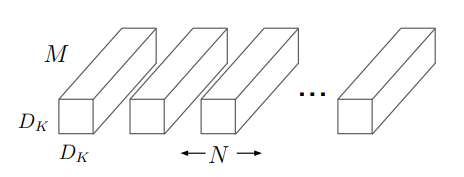
\includegraphics[scale=0.7]{img/standart_convolution.PNG}
  \caption{Standartinė sąsūka (\textit{standart convolution}).}
  \label{fig:standart_convolution}
\end{figure}

\begin{figure}[h!]
\centering
  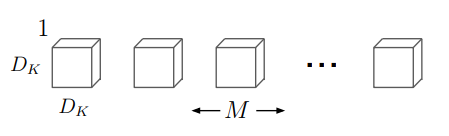
\includegraphics[scale=0.7]{img/depthwise_convolution.PNG}
  \caption{Gili sąsūką (\textit{depthwise convolution}).}
  \label{fig:depthwise_convolution}
\end{figure}

\begin{figure}[h!]
\centering
  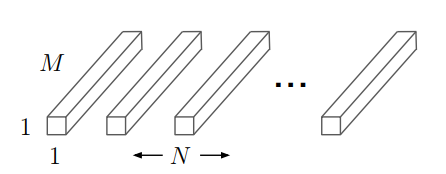
\includegraphics[scale=0.7]{img/pointwise_convolution.PNG}
  \caption{Giliai atskirta sąsūka (\textit{depthwise separable convolution}).}
  \label{fig:pointwise_convolution}
\end{figure}

\newpage

\subsubsection{Giliai atskiriama sąsuka (\textit{Depthwise Separable Convolution})}

Giliai atskiriama sąsūka yra gili (\textit{depthwise}) sąsūka, po kurios seka taškinė (\textit{pointwise}) sąsūka (Pav.\ref{fig:depthwise_conv2}).

\begin{figure}[h!]
\centering
  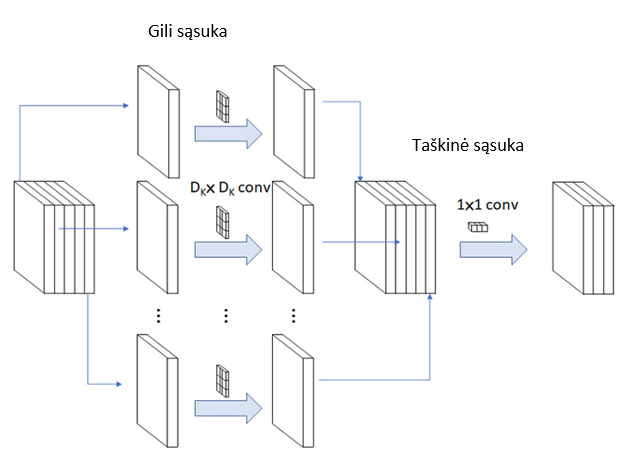
\includegraphics[scale=0.7]{img/depthwise_conv2.PNG}
  \caption{Giliai atskiriama sąsūka.}
  \label{fig:depthwise_conv2}
\end{figure}

\begin{itemize}
  \item Gili sąsūka yra kanalo dydžio D$_{K}$ × D$_{K}$ erdvinė sąsūka.
  \item Taškinė sąsūka iš esmės yra 1 × 1 filtras, skirtas dimensijai pakeisti.
\end{itemize}

Taigi operacijos kaina yra (giliai atskiriamos sąsūkos kaina: gilios sąsūkos kaina + taškinės sąsūkos kaina):

\[ D_K \times D_K \times M \times D_F \times D_F + M \times N \times D_F \times D_F \]

kur M: įvedimo kanalų skaičius, N: išvedimo kanalų skaičius, D$_{K}$: branduolio dydis, D$_{F}$: aktyvavimo žemėlapio (\textit{activation map}) dydis.

Standartinės sąsūkos atveju:

\[ D_K \times D_K \times M \times N \times D_F \times D_F \]

Taigi skaičiavimo sumažinimas yra:

\[ \dfrac{D_K \times D_K \times M \times D_F \times D_F + M \times N \times D_F \times D_F}{D_K \times D_K \times D_K  \times M \times N \times D_F \times D_F} = \dfrac{1}{N} + \dfrac{1}{D_K^2} \]

Kai D$_{K}$ × D$_{K}$ yra 3 × 3, galima pasiekti 8–9 kartus mažesnį skaičiavimų kiekį, tačiau su nedideliu tikslumo sumažinimu.

\newpage

\subsubsection{\textit{MobileNet} modelio architektūra}

Bendra \textit{MobileNet} architektūra yra sudaryta iš 30 sluoksnių\cite{10}:

\begin{enumerate}
  \item Sąsūkos sluoksnis su poslinkiu 2.
  \item Gilus (\textit{depthwise}) sluoksnis.
  \item Taškinis (\textit{pointwise}) sluoksnis, padvigubinantis kanalų skaičių.
  \item Gilus (\textit{depthwise}) sluoksnis su poslinkiu 2.
  \item Taškinis (\textit{pointwise}) sluoksnis, padvigubinantis kanalų skaičių.
  \item etc.
\end{enumerate}

\begin{figure}[h!]
\centering
  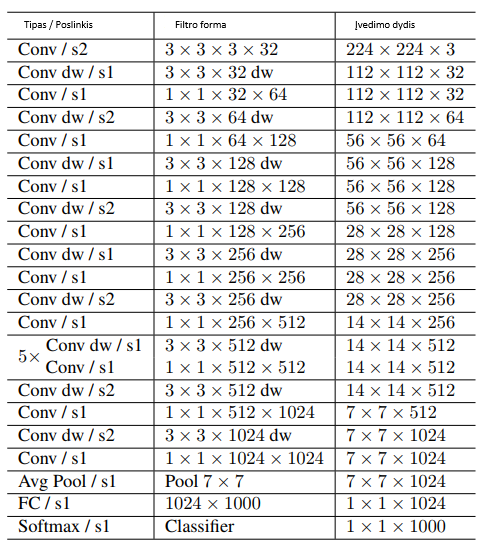
\includegraphics[scale=0.7]{img/mobilenet_table.PNG}
  \caption{\textit{MobileNet} tinklo pilna architektūra.}
  \label{fig:pointwise_convolution}
\end{figure}

\newpage
\subsection*{Išvados}

Atlikus darbą paaiškėjo, kad yra skirtingi būdai realizuoti gilųjį mokymą. Vienas iš jų yra panaudojant \textit{Keras} biblioteką, kuri yra  \textit{TensorFlow} apvalkalas. Šis būdas yra geriau žinomas ir dažniau naudojamas. \textit{Keras} turi daug naudingų funkcijų, kurios leidžia prieiti prie giliojo mokymosi problemų iš skirtingų pusių. Taip pat \textit{Keras} labai gerai tinka žmonėms, kurie nori pradėti naudoti gilųjį mokymą, kadangi \textit{Keras} neturi tokio didelio abstrakcijos lygio, kaip \textit{TensorFlow.js}, todėl žmogus turi suprasti ką naudoją ir iškviečia rašant programą su \textit{Keras}. Bet tuo pačiu metu \textit{Keras} yra pakankamai draugiškas vartotoju, palyginant su \textit{TensorFlow}. Vienas iš \textit{Keras} trūkumų palyginant jį su \textit{TensorFlow.js} yra įrangos nustatymas, kuris gali užimti nemažai laiko. Taip pat norint efektyviai apmokyti tinklą, reikia turėti pakankamai geras \textit{Python} žinias.
\par
\textit{TensorFlow.js} yra pakankamai naujas projektas, kol kas ne daug žmonių netgi žino apie jį. Dėl to, kad tai yra naujas projektas, jame trūksta pakankamai daug reikalingo funkcionalumo, pvz: vaizdų aktyvavimų išsaugojimo ir įkėlimo. Taip pat \textit{TensorFlow.js} nėra labai gerai optimizuotas -- apmokant tinklą panaudojant didesnį kiekį objektų, naršyklė negalėjo susitvarkyti su apmokytu tinklu. Nekreipiant dėmesio į trūkumus, \textit{TensorFlow.js} turi daug pranašumų. Jis turi didelį abstrakcijos lygį, kuris leidžia žmogui, kuris yra susipažinęs su giliuoju mokymusi, greitai sukurti ir apmokyti tinklą naršyklėje. Taip pat \textit{TensorFlow.js} turi pakankamai daug naudingo funkcionalumo. Vienas iš jų yra mokymosi perkėlimas, su kurio pagalba tinklą, kuri reikėtu mokyti porą valandų, galima apmokyti per pora minučių. Nekreipiant dėmesio į trūkumus, \textit{TensorFlow.js} yra projektas turintis daug potencialo, kuris ateityje taps vienu iš pagrindinių įrankių giliojo mokymosi srityje.
\par
Šiame darbe sukūrėme neuroninį tinklą, kuris atpažįsta \textit{„Lego“} detales su tikimybe 77\%, panaudojant \textit{Keras} biblioteką. Su \textit{ImageJ} pagalba panaudojom skirtingus būdus normalizuoti duomenų rinkinį. Po skirtingų normalizavimų būdų lyginome paveikslėlių histogramas. Toliau palyginome skirtingas neuroninio tinklo architektūras. Toliau sukonstravome neuroninį tinklą  \textit{TensorFlow.js} pagalba, kuris randa rankos poziciją vaizde ir atpažįsta rankoje laikomą objektą su tikimybe 75\%. Tinklo konstravimui naudojome mokymosi perkėlimą (\textit{Transfer learning}),  kurio pagalba apmokyti tinklą atpažinti objektą reikia kur kas mažiau apmokymo duomenų ir laiko. Rankos atpažinimui panaudojome \textit{HandTrack.js} biblioteką.

\newpage

\subsection*{Santrauka}

Šiame darbe konstravome neuroninius tinklus naudojant \textit{Keras} ir \textit{TensorFlow.js} bibliotekas. Konstruojant neuroninį tinklą, kuris galėtu atpažinti skirtingas \textit{„Lego“} detales, su \textit{Keras}, bandėme normalizuoti duomenų rinkinį ir palyginti skirtingas tinklo architektūras. Konstruojant tinklą, kurį galėtume apmokyti atpažinti skirtingus rankoje laikomus objektus, su \textit{TensorFlow.js}, panaudojom mokymo perkėlimą, su kurio pagalba tinklo apmokymui prireikė kur kas mažiau laiko ir apmokymo duomenų.

\subsection*{Summary}

In this work we have constructed neural networks using Keras and TensorFlow.js libraries. By constructing a neural network, that could recognize different Lego pieces, with Keras, we tried to normalize the data set and compare different network architectures. Using a TensorFlow.js library to construct a neural network, that could be trained to recognize different hand-held objects, we used a training transfer that made network training less time-consuming and also require less training data.

\newpage


\addcontentsline{toc}{section}{Literatūra}

\begin{thebibliography}{9}

\bibitem{Deep Learning with Python} 
Francois Chollet. 
\textit{Deep Learning with Python}. 
October 28, 2017.
\\\texttt{https://www.manning.com/books/deep-learning-with-python}

\bibitem{Keras documentation} 
\textit{Keras documentation}.
\\\texttt{https://keras.io/}

\footnotesize
\bibitem{Convolutional neural networks with keras} 
\textit{Convolutional neural networks with keras}.
\\\texttt{https://cambridgespark.com/content/tutorials/convolutional-neural-networks-with-keras/}

\bibitem{Keras Functional API for Deep Learning} 
\textit{Keras Functional API for Deep Learning}.
\\\texttt{https://machinelearningmastery.com/keras-functional-api-deep-learning/}

\bibitem{Applications of Deep Learning} 
\textit{Applications of Deep Learning}.
\\\texttt{https://machinelearningmastery.com/inspirational-applications-deep-learning/}

\bibitem{ImageJ API} 
\textit{ImageJ API}.
\\\texttt{https://imagej.nih.gov/ij/developer/api/index.html}

\bibitem{Writing ImageJ Plugins-A Tutorial} 
\textit{Writing ImageJ Plugins-A Tutorial}.
\\\texttt{https://media.ijm.fr/fileadmin/www.ijm.fr/MEDIA/imagerie/fichiers/tut\_pluginwb.pdf}

\bibitem{Image Data Pre-Processing for Neural Networks} 
\textit{Image Data Pre-Processing for Neural Networks}.
\\\texttt{https://becominghuman.ai/image-data-pre-processing-for-neural-networks-498289068258}

\bibitem{TensorFlow.js documentation} 
\textit{TensorFlow.js documentation}.
\\\texttt{https://www.tensorflow.org/js}

\bibitem{MobileNets: Efficient Convolutional Neural Networks for Mobile VisionApplications} 
Andrew G. Howard.
\textit{MobileNets: Efficient Convolutional Neural Networks for Mobile VisionApplications}.
April 17, 2017.
\\\texttt{https://arxiv.org/pdf/1704.04861.pdf}

\bibitem{Handtrack.js: Hand Tracking Interactions in the Browser using Tensorflow.js} 
\textit{Handtrack.js: Hand Tracking Interactions in the Browser using Tensorflow.js}.
\\\texttt{https://hackernoon.com/handtrackjs-677c29c1d585}

\bibitem{Get to know TensorFlow.js} 
\textit{Get to know TensorFlow.js}.
\\\texttt{https://medium.freecodecamp.org/get-to-know-tensorflow-js-in-7-minutes-afcd0dfd3d2f}

\bibitem{JavaScript for Machine Learning using TensorFlow.js} 
\textit{JavaScript for Machine Learning using TensorFlow.js}.
\\\texttt{https://blog.bitsrc.io/javascript-for-machine-learning-using-tensorflow-js-6411bcf2d5cd}

\end{thebibliography}









\end{document}
